% Copyright (c) 2024, Francisco Fernandez
% License: CC BY-SA 4.0
%   https://github.com/fernandezfran/thesis/blob/main/LICENSE
\section{Introducción}

Dentro de la industria de vehículos eléctricos, la carga rápida es una de las principales características a ser 
mejorada. Para dar una idea del desafío con el cual nos encontramos, cabe mencionar que el tiempo 
de recarga de la batería de los autos eléctricos de Nivel 2 se encuentra entre 
las 4 y las 10 horas \cite{evcs}. Este número es dos órdenes de magnitud 
mayor que el tiempo que toma recargar un auto a combustión interna.

Existen distintos criterios para definir que una carga sea rápida. Uno de ellos, 
pensado para la aplicación de vehículos eléctricos, aspira lograr una autonomía de 30 km 
por minuto de carga \cite{dufek2022}. Otro criterio, definido por el USABC (de sus
siglas en inglés, \textit{United States Advanced Battery Consortium}), tiene como
objetivo obtener el 80\% del Estado de la Carga (SOC, \textit{State-of-Charge})
en 15 minutos \cite{USABC}. Este último es el criterio elegido para esta tesis.
Para cumplir con el mismo, es necesario entender la física de los materiales de
intercalación y cómo estos se comportan durante el cargado, ya que esto podría 
permitir una optimización en el diseño de los electrodos.

La carga rápida es un problema multi-escala \cite{franco2013, franco2019} y, por 
lo tanto, las mejoras en la velocidad de carga de las celdas electroquímicas 
requieren de una comprensión desde el nivel atómico hasta el ingenieril. Dentro 
de lo que es la escala micrométrica, los procesos que determinan la velocidad de 
carga al nivel de una sola partícula de los materiales de electrodos son la 
difusión de iones de litio dentro de electrodos y la transferencia de carga en 
la interfase electrodo/electrolito, por lo cual es necesario favorecer ambos
procesos \cite{liu2019, tomaszewska2019, weiss2021}. También se ha estudiado la 
importancia del rol del tamaño y la geometría de las partículas en el desempeño 
electroquímico \cite{gavilan2020, gavilan2022}. Así, incluso descartando
otros factores que podrían influir en la carga de la batería (como los cambios de 
volumen durante la intercalación de iones de litio, las características termodinámicas particulares
de los sistemas, la formación de interfase electrolito/sólido, etc), es complicado
realizar un análisis detallado del desafío general que representa este problema.

La electroquímica de electrodos de una sola partícula \cite{ventosa2021, 
heubner2020, takahashi2020, wahab2020, xu2020, tao2019, fukui2011} permite 
estudiar la respuesta \say{pura} de los materiales activos, esto es, sin el efecto 
de otros aditivos presentes en los electrodos compuestos. Esta información 
detallada es valiosa, ya que da a conocer los factores limitantes para su 
carga rápida y su respuesta frente a la misma. Enmarcado en este contexto, en 
este capítulo se utiliza un modelo de una sola partícula que fue introducido en la 
sección \ref{s:metodologia}.

Las relaciones de escaleo suelen dar una respuesta simple, aunque aproximada, a 
problemas complejos, esta cualidad ha hecho que tengan una gran popularidad 
en la física y en la química. Quizás uno de los casos más conocidos sea el de los
gases ideales
\begin{equation}
    \frac{p V}{n T} = R,
\end{equation}
que no es más que escalear el producto de la presión y el volumen, $p V$, por la
temperatura absoluta, $T$, y el número de moles, $n$, para obtener una constante
universal. Aunque de forma aproximada, esta ecuación proporciona una guía 
importante para resolver muchos problemas prácticos y es utilizada como referencia
para entender el comportamiento de fluidos más complejos que los gases ideales.

Dentro de esta perspectiva, en un trabajo reciente se ha propuesto una figura de mérito que permite establecer 
una jerarquía entre distintos materiales de carga rápida \cite{xia2022}. 
Esta consiste en combinar los efectos de los coeficientes de difusión y los 
tamaños geométricos para definir el tiempo característico de difusión, 
$\tau = d^2 / D$, y es presentada en la Figura \ref{fig:xiafom}. Esta figura de 
mérito supone un sólido semi-infinito y una reacción interfacial ultrarrápida, 
es decir que supone que el proceso limitante es la difusión de los iones dentro 
del material.
\begin{figure}[h!]
    \centering
    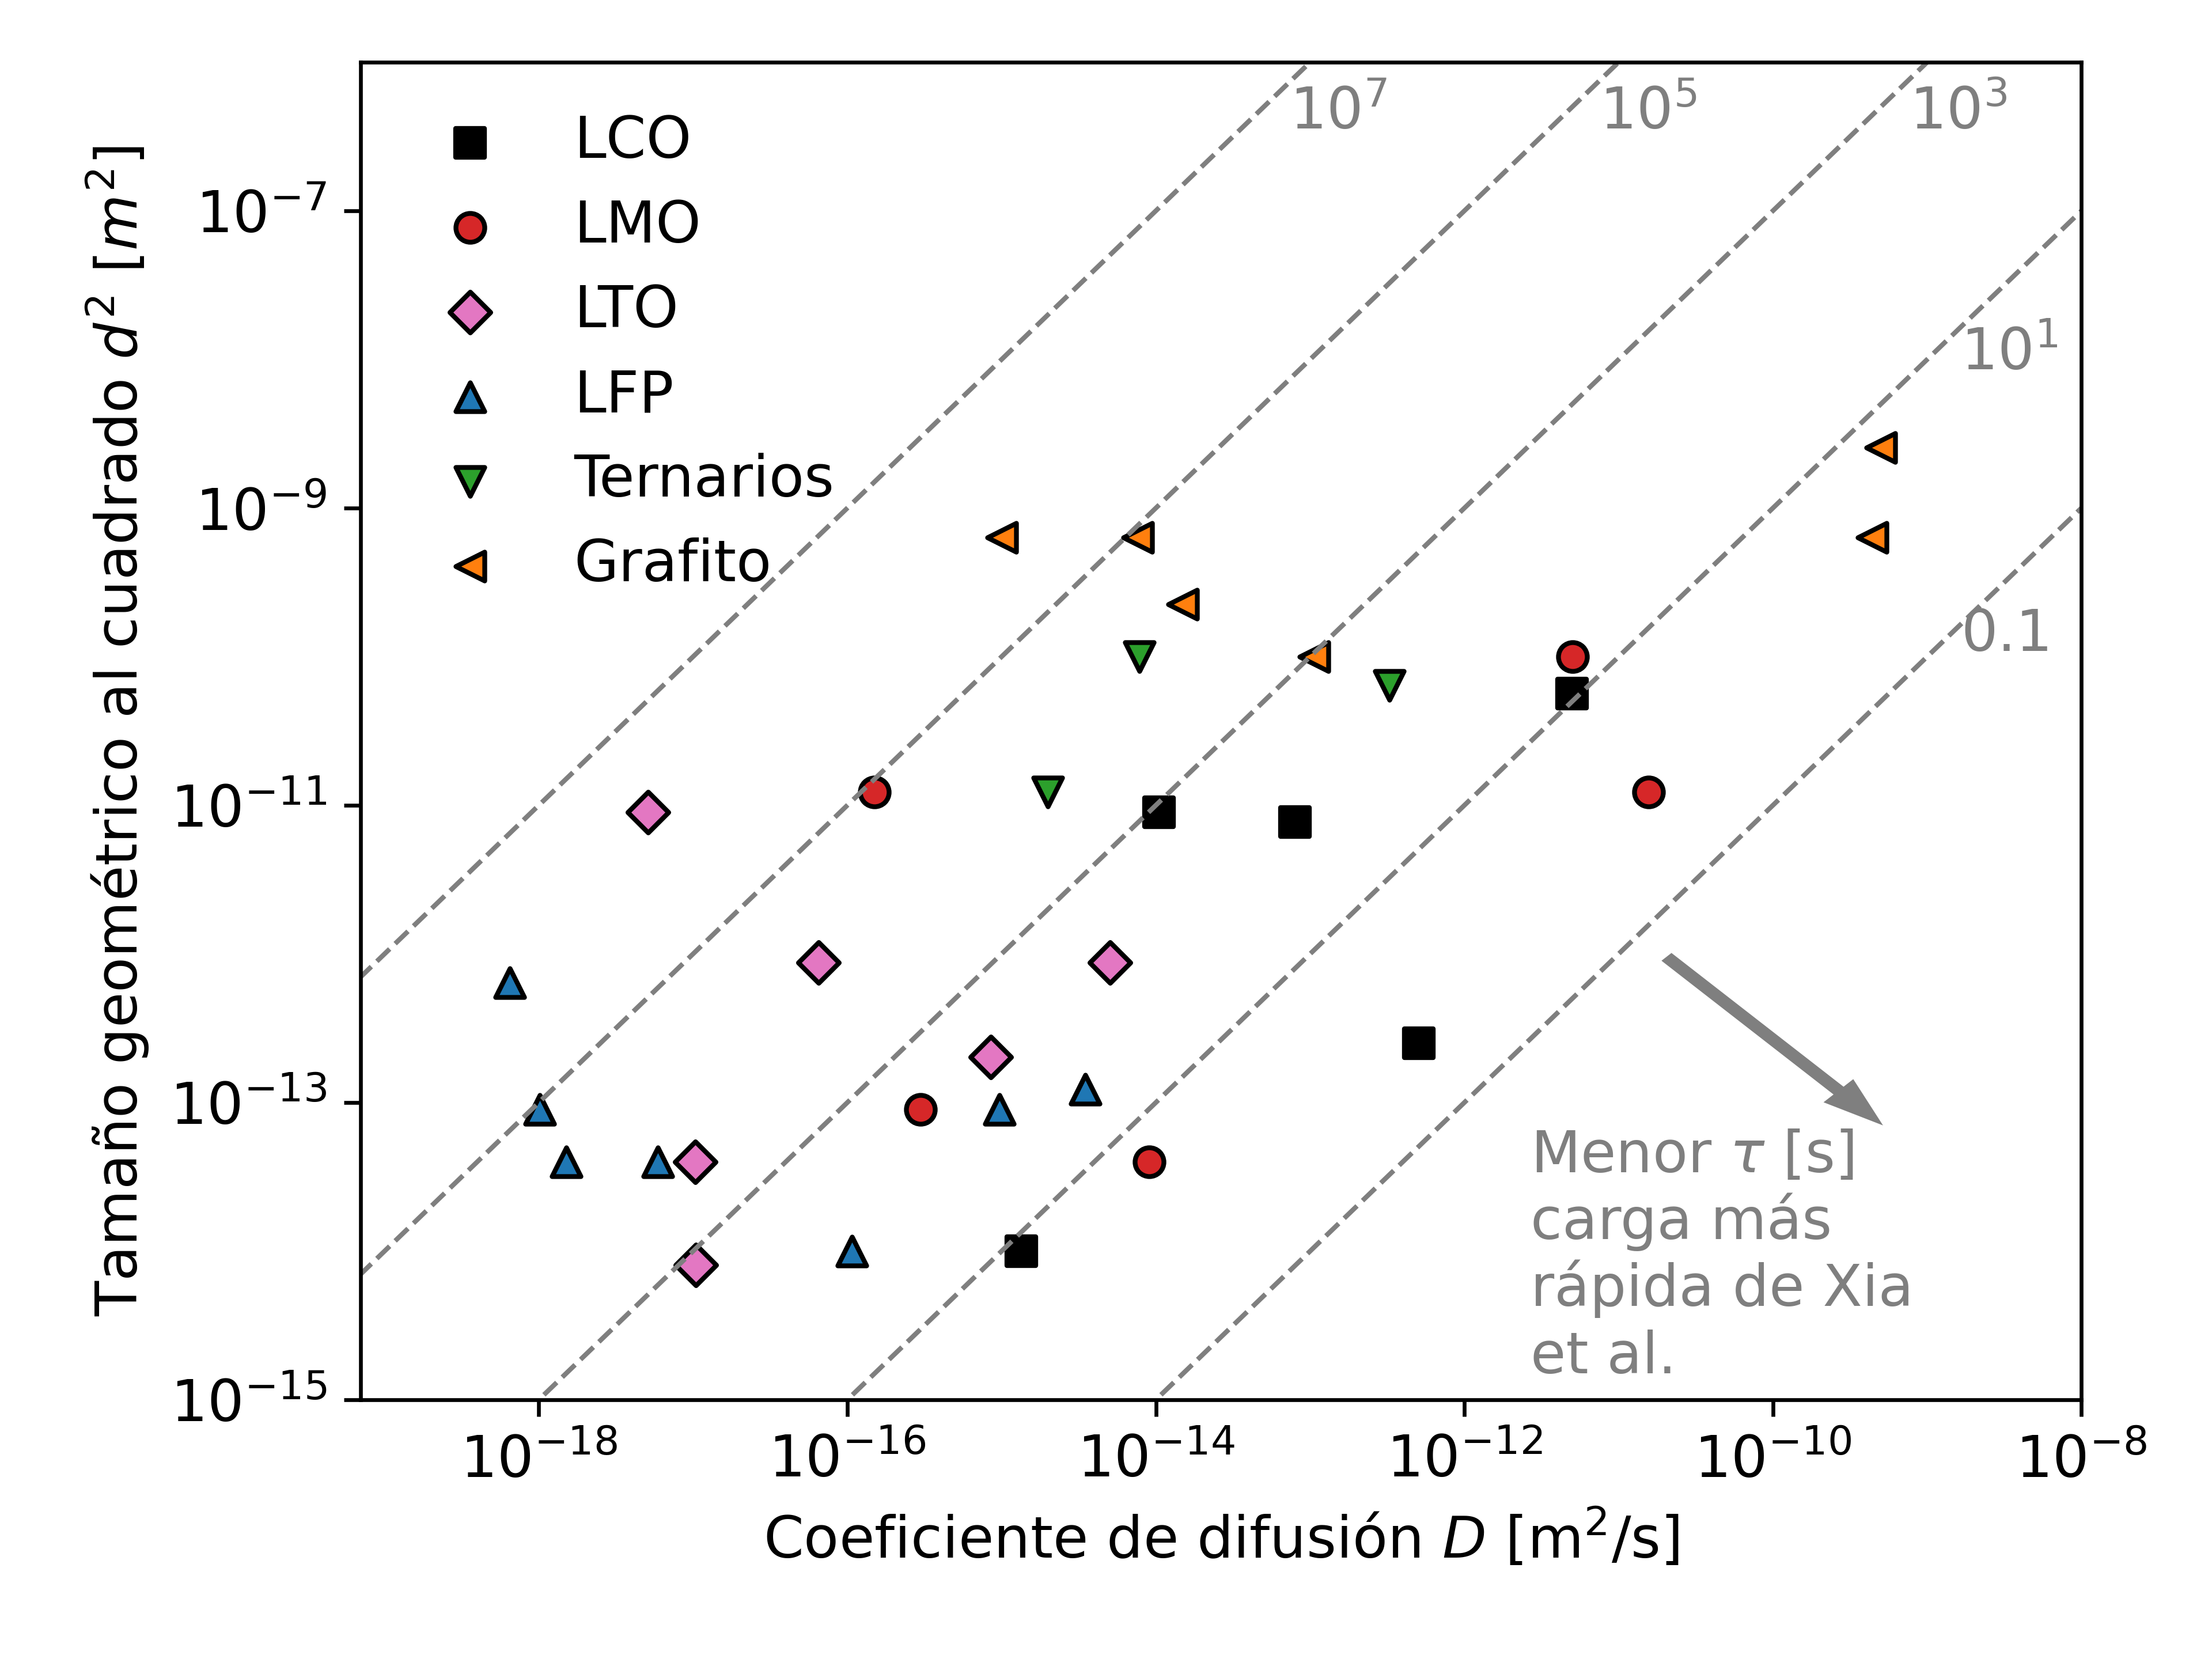
\includegraphics[width=.7\textwidth]{FastCharging/un/introduccion/xiafom.png}
    \caption{Figura de mérito definida como el tiempo característico de difusión, 
    $\tau = d^2/D$, propuesta por Xia \textit{et al.} \cite{xia2022}. La líneas
    grises discontinuas indican valores de $\tau$ constantes que dividen a los 
    materiales en clases con diferentes capacidades de carga rápida.}
    \label{fig:xiafom}
\end{figure}
Extendiendo estas consideraciones, el modelo de una sola partícula que se utiliza 
aquí además de considerar el coeficiente de difusión y el tamaño de la partícula,
también tiene en cuenta la constante cinética en la interfase y la velocidad 
de carga galvanostática (C-rate) en dos parámetros adimensionales: 
uno cinético, $\Xi = k^0 \sqrt{\frac{t_h}{C_r D}}$ (ecuación \ref{eq:xi}), 
y el otro de difusión finita, $\ell = d \frac{V}{A} \frac{C_r}{D t_h}$
(ecuación \ref{eq:ele}), que pueden emplearse para construir
diagramas galvanostáticos de la capacidad máxima alcanzada a un dado potencial
de corte, SOC$_{\max}$. Estos parámetros $\Xi$ y $\ell$ son relaciones de escaleo útiles
para realizar una primera predicción cualitativa de la capacidad que un 
material alcanzaría a una dada C-rate. Esto es relevante, ya que permite
realizar la tarea no-trivial de clasificar distintos materiales, cada uno 
caracterizado por los descriptores $D$, $k^0$ y $d$. Se ha demostrado \cite{gavilan2022} que la capacidad de carga máxima que un material puede alcanzar en el cargado galvanostático hasta un dado sobrepotencial, SOC$_{\max}$, 
puede expresarse como una función universal de dichos parámetros de escaleo $\Xi$ y $\ell$,
\begin{equation}\label{eq:socmax}
    \text{SOC}_{\max} = f(\Xi, \ell) = f(d, D, k^0, C_r).
\end{equation}
Estos valores se ilustran en las Figuras \ref{fig:diagnostico}b y \ref{fig:diagnostico}c como triángulos marcados en las abcisas.
Como no se tiene una expresión análitica para esta función $f$, la misma puede ser 
obtenida en un mapeo ($\Xi$, $\ell$) de simulaciones galvanostáticas, como se la 
presenta en la Figura \ref{fig:diagnostico}a en un gráfico de colores de dos 
dimensiones. Dicho mapa se construye con los cortes con el eje de las abscisas de los perfiles galvanostáticos
al potencial de corte de 150 mV debajo del potencial de equilibrio (en las Figuras 
\ref{fig:diagnostico}b y c se presentan ejemplos para algunos valores particulares 
de $\Xi$ y $\ell$).
\begin{figure}[h!]
    \centering
    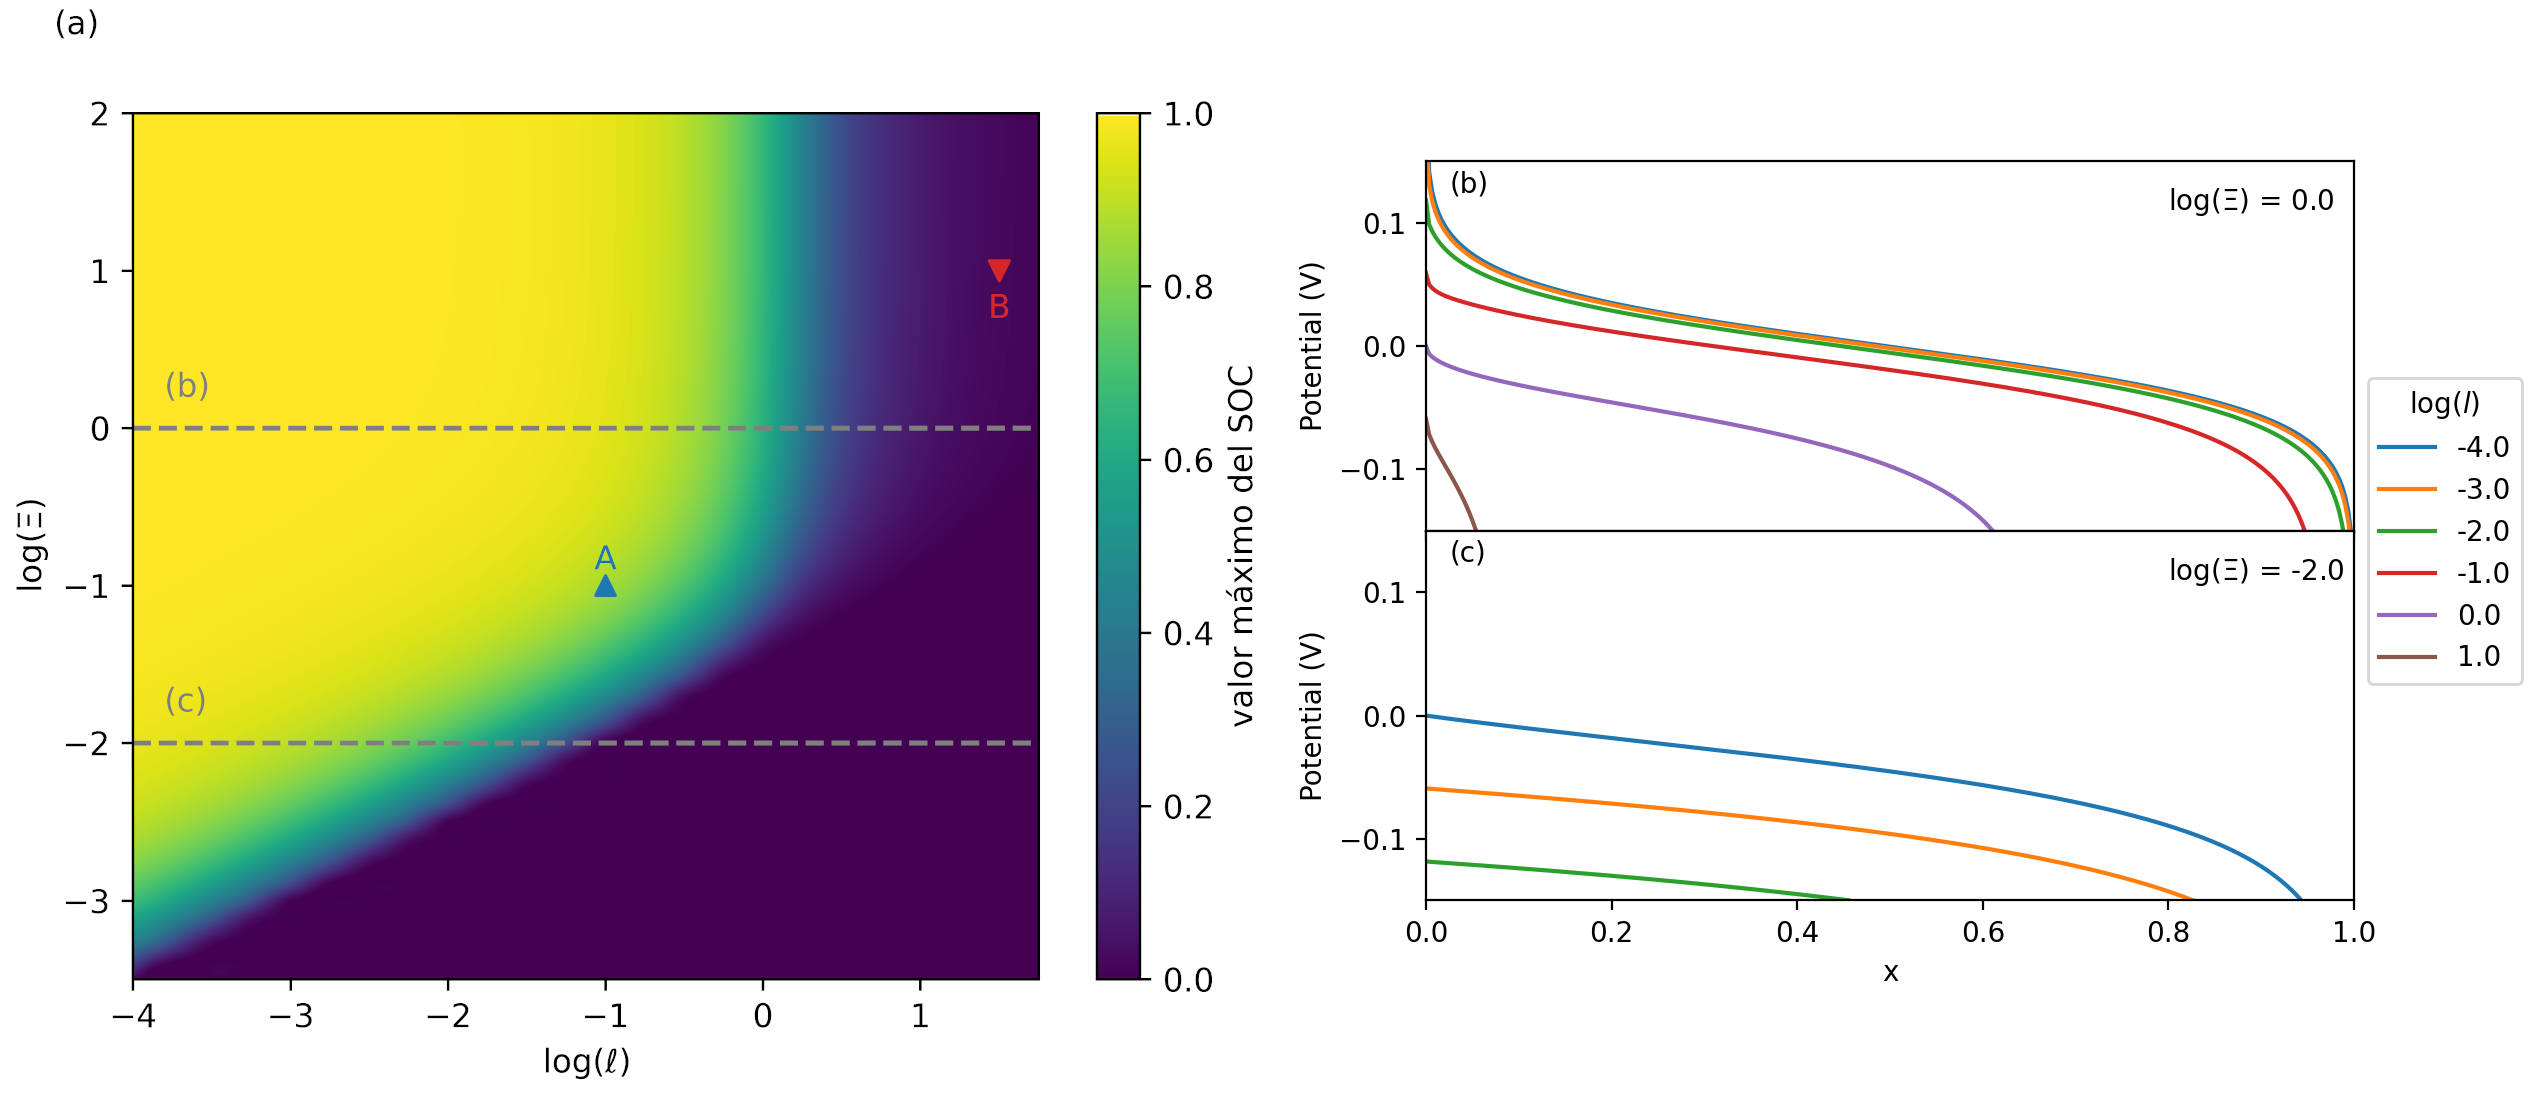
\includegraphics[width=\textwidth]{FastCharging/un/introduccion/diagnosis-merged.png}
    \caption{(a) Diagrama de nivel para una geometría esférica con un voltaje de 
    corte de 150 mV y condiciones de contorno detalladas en la sección 
    \ref{s:metodologia}. Los datos de los puntos A y B se encuentran en la 
    Tabla \ref{t:ab}. (b) y (c) muestran perfiles voltaje/capacidad para 
    diferentes valores particulares de $\Xi$ y $\ell$ (ver líneas grises 
    discontinuas en la Figura \ref{fig:diagnostico}a), los triángulos negros 
    sobre el eje SOC indican los valores de SOC$_{\max}$ alcanzados.}
    \label{fig:diagnostico}
\end{figure}

Desde el punto de vista del trabajo de Xia \textit{et al.} \cite{xia2022}, 
la ecuación \ref{eq:socmax} evaluada en el punto ($\Xi$, $\ell$) también puede 
introducirse como una figura de mérito. Supongamos que 
tenemos dos materiales, A y B, con las propiedades dadas en la Tabla \ref{t:ab} y 
se quiere determinar si alguno de ellos es un buen candidato para una carga en 15 
minutos.
\begin{table}[h!]
    \centering
    \caption{Ejemplo de dos materiales, A y B, caracterizados por sus coeficientes 
    de difusión, sus constantes cinéticas y sus tamaños.}
    \setlength\extrarowheight{2pt}\stackon{%
    \begin{tabular}{l c c c c c}
        \toprule
        \textbf{Material} & 
        \textbf{$D$ [cm$^2$/s]} &  
        \textbf{$k^0$ [cm/s]} &
        \textbf{$d$ [cm]} &  
        \textbf{$\log(\Xi)$} & 
        \textbf{$\log(\ell)$} \\
        \midrule
        A & 3.7$\times 10^{-9}$ & 2.03$\times 10^{-7}$ & 0.001 & -1.0 & -1.0 \\
        B & 1.17$\times 10^{-11}$ & 1.14$\times 10^{-6}$ & 0.001 & 1.5 & 1.0 \\
        \bottomrule
    \end{tabular}
    }{}
    \label{t:ab}
\end{table}
Entonces, con los datos de las columnas 2--4 de la Tabla \ref{t:ab} 
se pueden calcular los valores de $\Xi$ y $\ell$, utilizando las ecuaciones 
\ref{eq:xi} y \ref{eq:ele}, presentados en la quinta y la sexta columna de la 
Tabla \ref{t:ab}. Los puntos correspondientes a estos materiales se presentan en 
el mapa de la Figura \ref{fig:diagnostico}a. A partir de este, podemos ver que el 
material A es un buen candidato para una carga en 15 minutos mientras que el 
material B no lo es.

El principal objetivo de este capítulo es proponer que estos diagramas generales 
sean utilizados con un enfoque heurístico, aprovechando datos experimentales de la
literatura, para mostrar que pueden proporcionar una guía simple y rápida para 
estudiar la cinética y el comportamiento de materiales específicos bajo 
condiciones de carga rápida.
